%!TEX root = Zusammenfassung.tex

\section{Verfahren via CfFada}
CfFada heißt ausgeschrieben \glqq Controllflow based Fuzzy array dataflow\grqq.\\
Dieses weiteres Verfahren wird motiviert durch die Existenz von \glqq if-Statements\grqq\ , \glqq unstrukturierte Programme\grqq\ und die erhöhte \glqq Präzision\grqq.


\subsection{Idee}
\begin{enumerate}
\item Zusammenführen von
  \begin{enumerate}
  \item traditionellen (universell einsetzbar, ungenau) und
  \item einem Feautrier-ähnlichem Verfahren
  \end{enumerate}
\item (Effizienz)
\end{enumerate}


\subsection{Prinzipielles Vorgehen}
\begin{enumerate}
\item Konstruiere den Kontrollflußgraphen (CFG)
\item Für jeden Zugriff $a$:
  \begin{enumerate}
  \item Annotiere den CFG mit den für a relevanten Relationen - unter Berücksichtigung der umgebenden Prädikate
  \item starte mit leerer Abhängigkeitsmenge (alles bottom) und Ordnungsrelation $(=,...,=)$ bei a. (\( i = i^\prime = \dots \))
  \item durchlaufe den CFG rückwärts
  \item bei Schleifen: durchlaufe die Rückwärtskanten von innen nach außen und passe die aktuell gültige Ordnungsrelation an
  \item bei \glqq conflicting accesses\grqq : mische die neuen und alten Abhängigkeiten unter Berücksichtigung der Optimierung
  \end{enumerate}
\end{enumerate}


\subsection{Anmerkungen}
\begin{enumerate}
  \item Implementierung mit Omega (Presburger Arithmetik) \( \rightarrow \) Genauigkeit
  \item unstrukturierte Programme \( \rightarrow \) Abschätzung der Ordnungsrelation
  \item vorzeitiges Analyse-Ende möglich, wenn alle möglichen letzten Quellen gefunden wurden.
  \item Der Hauptunterschied zu Feautrier besteht in der Tatsache, dass CfFada mit if-Statemants umgehen kann.
  \item textuell getragene Abhängigkeiten entspricht sprachlich den Schleifenunabhängigen Abhängigkeiten
  \item Mischen: Schneiden und Optimierung
  \item \( \Box := \) Merge/Mischen
  \item \( W(6) := \) Write-Set von 6
\end{enumerate}


\subsection{Beispiel}
\begin{figure}[h]
    \begin{subfigure}[c]{.5\linewidth}
        \paragraph{Programmcode}~\\
        \begin{procedure}[H]
        \SetAlgoLined
        \For{$i=0$ \KwTo $N$}{
            \For{$j=0$ \KwTo $N$}{
                \textbf{3:} $A[i+j+1]$ = ... \\
                \eIf{$P$}
                    {\textbf{6:} $A[i+j]$ = ...\\}{}
                \textbf{7:} ... = $A[i+j]$
            }
        }
        \end{procedure}
        \caption{Programmcode}
    \end{subfigure}
    \begin{subfigure}[c]{.5\linewidth}
        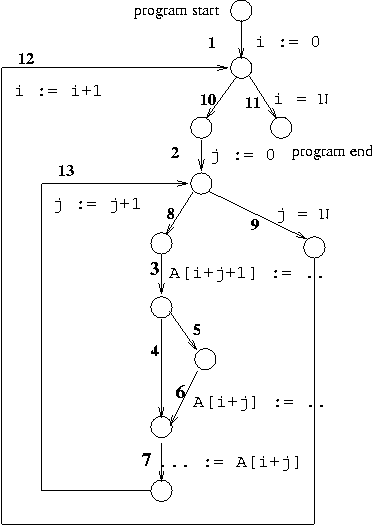
\includegraphics[width=\linewidth]{images/cffada.png}
        \caption{Ablaufgraph}
    \end{subfigure}
\end{figure}

\paragraph{Kontext}~\\
Read-Statement 7\\
Operationen: $\langle (i,j), 7 \rangle$ für $0 \leq i, j \leq N$

\paragraph{Annotierung}~\\
Statement 3\\
Operationen: $\langle (i^\prime,j^\prime), 3 \rangle\) für \( \underbrace{0 \leq i^\prime, j^\prime \leq N}_{Existenz} \land \underbrace{i^\prime + j^\prime + 1 = i + j}_{Konflikt}$\\
Statement 6\\
Operationen: \dots\\

\paragraph{Durchlauf}~\\
\begin{enumerate}
    \item {Ordnung: \(i=i^\prime \land j=j^\prime\) \\
        \(src^{(0)} = {\perp}\)\\
        \begin{enumerate}
            \item Start: 7
            \item die 4 hoch: (Kante mit Label 4)\\
                  Keine neuen Quellen\\
                  \(scr_{4}^{(1)} = \lbrace \perp \rbrace\)
            \item die 6 hoch: (überprüfe Existenzun- und Konfliktgleichungen)\\
                  \(src_{6}^{(1)} = src^{(0)} \Box W(6) = \)
    \(\begin{cases}  \langle (i,j), 6 \rangle , & \mbox{ für } P^\prime(i,j) \\
                     \perp ,                    & \mbox{ sonst }
    \end{cases}  \)

            \item bei n1 Mischen:\\
                \(scr_{n1}^{(1)} =
    \begin{cases} \langle (i,j),6 \rangle, & \mbox{ für } p^\prime(i,j) \\
                  \perp,                   & \mbox{ sonst }
                \end{cases} \)

            \item die 3 hoch:\\
                  Keine neuen Quellen, da die aktuelle Ordnung $\lightning$ Konfliktgleichung. (Wäre P immer true, könnte man an n1 abbrechen.)
            \item die 13 hoch \(\Rightarrow\)

        \end{enumerate}
        }
    \item {Ordnung: \(i=i^\prime \land j^\prime < j\) \\
      \begin{enumerate}
         \item die Kanten 7, 4 bringen nichts neues.
         \item die 6 hoch: \\
           Keine neuen Quellen, da die aktuelle Ordnung $\lightning$ Konfliktgleichung.
         \item n1: nichts neues zu mischen \(\Rightarrow\) alles bleibt
         \item die 3 hoch: \\
           \(src^{(2)} = src^{(1)} \Box W(3) = \) \\ \( =
           \begin{cases} \langle ( i^\prime, j^\prime), 3) \rangle, & \mbox{ für } i^\prime + j^\prime + 1 = i + j \land \neg P^\prime(i,j) \land 0 \leq i^\prime \leq N \land 0 \leq j^\prime \leq N \\ & \mbox{ mit aktueller Ordnung}\\
             \langle (i,j),6 \rangle , & \mbox{ für } P^\prime(i,j) \\
             \perp, & \mbox{sonst}
           \end{cases}
\)
           \\ \(\stackrel{j^\prime+1=j}{=}
           \begin{cases}
             \langle ( i, j-1), 3 \rangle, & \mbox{ für }\neg P^\prime(i,j) \land j > 0 \land 0 \leq j-1 \leq N \\
             \langle (i,j),6 \rangle , & \mbox{ für } P (i,j) \\
             \perp , & \mbox{ sonst, d.\,h. } j = 0 \land \neg P(i,0)
           \end{cases}
           \)
         \item Kante 8: -
         \item Kante 2: -
         \item Kante 10: -
         \item Kante 12: -
      \end{enumerate}
      }

      \item {Ordnung: \(i^\prime < i, j^\prime\) beliebig
          \begin{enumerate}
            \item Kante 9,13,7,4: -
            \item Kante 6: \\
              wegen Optimierung: \(j= 0 \land \neg P^\prime (i,j)\) \\
              Ordnung: \(i^\prime < i \) \\
              Konflikt: \( i^\prime + j^\prime = i + 0 \) \\
              Existenz: \( P^\prime(i^\prime, j^\prime) \) \\
              neue Quellen: \( \langle ( i^\prime, i-i^\prime ), 6 \rangle \text{ für } j=0, i^\prime < i , P(i^\prime, i - i ^\prime) \land \neg P(T, i-T) \text{ für } i^\prime < T \leq i \) \\

\( src^{(3)}_{n1} =
\begin{cases}
  \langle (i,j), 6 \rangle, & \mbox{ für } P(i,j) \\
  \langle (i,j-1), 3 \rangle, & \mbox{ für } j \geq 1 \land \neg P (i,j) \\
  \langle (i^\prime, i-i^\prime),6 \rangle, & \mbox{ für } j=0 \land i^\prime < i \land P(i^\prime, i - i^\prime) \land \neg P(T,i-T) \\ & \mbox{ für } i^\prime < T \leq i \land i^\prime \geq 0 \land i \geq 1 \\
  \perp, & \mbox{ für } j=0 \land \neg P(i^\prime, i - i^\prime) \text{ für alle } 0 \leq i^\prime \leq i
\end{cases} \)

\item Kante 3:\\
  wegen Optimierung: \( i^\prime = i - 1, j=0 \stackrel{Konfl. Gl.}{\Rightarrow} j^\prime = 0\) \\
  neue Quelle: \( \langle (i-1,0), 3 \rangle \text{für} j=0 \land i \geq 1 \land \neg P(i,0) \land \neg P(i-1,1) \) \\
\( \Rightarrow src =
\begin{cases}
  \langle (i, j), 6 \rangle, & \mbox{für } P(i,j) \\
  \langle (i, j-1), 3 \rangle, & \mbox{für } j \geq 1 \land \neg P(i,j) \\
  \langle (i-1, 1), 6 \rangle, & \mbox{für } j=0 \land \neg P(i,j) \land P(i-1,1) \\
  \langle (i-1, 0), 3 \rangle, & \mbox{für } j=0 \land \neg P(i,j) \land \neg P(i-1,1) \land i \geq 1 \\
  \perp, & \mbox{für } i=j=0 \land \neg P(0,0)
\end{cases}
\)
\item Kanten 8, 2, 10, 1: -
           \end{enumerate}
           }

\end{enumerate}
Da die Quelle für \( (0,0) \) nicht gefunden wird, kann nicht vorab abgebrochen werden und der Algorithmus terminiert erst mit dem vollständigen Durchlauf.
